\documentclass[12pt]{report}
%\usepackage[a4paper, total={15cm, 20cm}]{geometry}

\usepackage{amsmath}
\usepackage{amsthm}
\usepackage{amssymb}
\usepackage{graphicx}
\usepackage{natbib}
\usepackage{url}
\usepackage{subcaption}
\usepackage[nottoc]{tocbibind}

\DeclareMathOperator{\expfamily}{ExpFamily}
\DeclareMathOperator{\expectation}{E}
\DeclareMathOperator{\variance}{Var}
\DeclareMathOperator{\cov}{Cov}
\DeclareMathOperator{\corr}{Corr}
\DeclareMathOperator{\bernoulli}{Bernoulli}
\DeclareMathOperator{\betaDist}{Beta}
\DeclareMathOperator{\dirichlet}{Dir}
\DeclareMathOperator{\bin}{Bin}
\DeclareMathOperator{\MN}{Multinomial}
\DeclareMathOperator{\prob}{P}
\DeclareMathOperator{\trace}{Tr}

\newcommand{\RSS}{\mathrm{RSS}}
\newcommand{\euler}{\mathrm{e}}
\newcommand{\diff}{\mathrm{d}}
\newcommand{\T}{^\textup{T}}
\newcommand{\dotdotdot}{_{\phantom{.}\cdots}}

\newcommand{\vect}[1]{\mathbf{#1}}
\newcommand{\vectGreek}[1]{\boldsymbol{#1}}
\newcommand{\matr}[1]{\mathsf{#1}}

\newtheorem{theorem}{Theorem}
\newtheorem{algorithm}{Algorithm}


\begin{document}

%=====TITLE PAGE======
\begin{titlepage}
\centering
\vspace*{1cm}
        
        \LARGE
        \textbf{Inside-Out: Characterisation of Computed Tomography Noise in Projection and Image Space with Applications to 3D Printing}
        
		\large        
        
        \vspace{2cm}
        {OxWaSP 2015 Warwick Cohort - Mini-project 1}
        
        \vspace{1cm}
        {Sherman Ip}

        \vspace{1cm}
        {Supervisor: Dr.~J.~Brettschneider (Statistics, Warwick)}
        
        \vspace{1cm}
        {Supervisor: Prof.~T.~Nichols (Statistics, Warwick)}
        
        \vspace{1cm}
        {10th June 2016}
\end{titlepage}

%======ABSTRACT=========
\begin{abstract}
I did this. This happened. I should of done that.
\end{abstract}

%======ACKNOWLEDGEMENT=========
\renewcommand{\abstractname}{Acknowledgements}
\begin{abstract}
None
\end{abstract}

%=====FRONT MATTER=====
\tableofcontents
%\listoffigures
%\listoftables

%======INTRODUCTION========
\chapter{Introduction}
Mini-project for OxWaSP.

%======LITERATURE REVIEW========
\chapter{Literature Review}
Computed tomography (CT) scanning is a 3D imaging technique. It does this by reconstructing the geometry of the sample through a series of 2D X-ray images of the sample. The sample rotates after each image taken.

Figure \ref{fig:x_ray_ct} shows a diagram on how CT scanning works. A 2D image is taken by projecting X-ray photons onto the stationary sample. The photons are then scattered or absobred by the sample.  Some of these photons are then detected by an X-ray detector on the other side of the sample, which produces an image. After an image has been taken, the object rotates and another image is taken. Finally after a number of images, a 3D reconstruction of the object can be estimated \cite{cantatore2011introduction}.

\begin{figure}
\centering
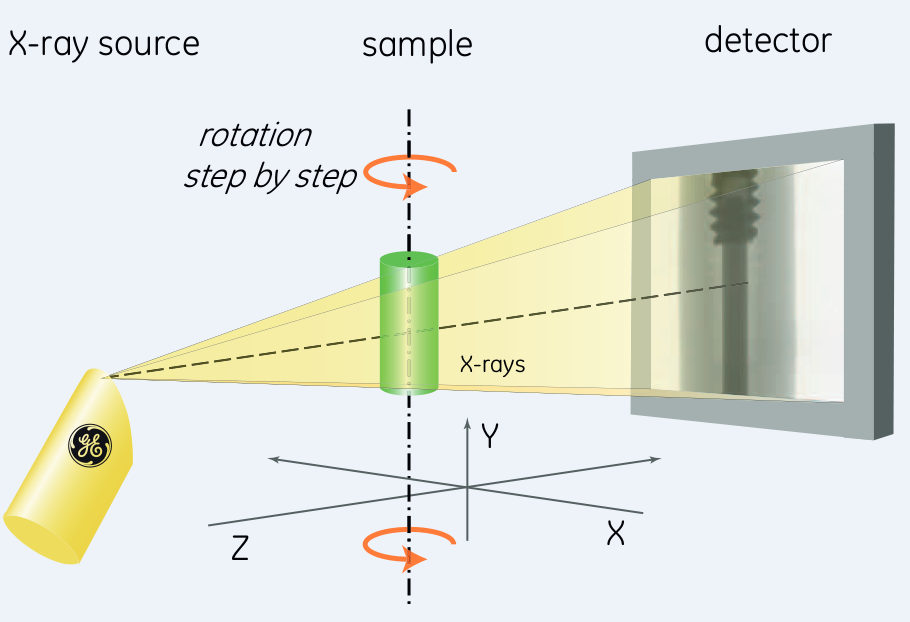
\includegraphics[width=0.7\textwidth]{figures/x_ray_ct.png}
\caption{X-ray computed tomography reconstructs the sample by projecting X-ray photons onto a rotating sample. The photon are then detected by the detector. \emph{Source: http://www.phoenix-xray.com/}}
\label{fig:x_ray_ct}
\end{figure}

CT scanning was invented by G. Hounsfield \cite{hounsfield1980computed} in the 1980's and it was mainly used for medical imaging. The setup for CT scanning is different when scanning patients because the detector and X-ray source rotates around the patient \cite{cantatore2011introduction}. Recently CT has been used industrially for non-destructive testing in manufacturing \cite{cantatore2011introduction}. One possible application would be inspecting 3D printed (additive layer manufactured) samples.

There are many sources of error in CT scanning \cite{cantatore2011introduction} and this can cause problems when reconstructing the geometry of the sample. Sources of error include: defects in the detector, environmental noise and the behaviour of photons.

This chapter aims to give brief description on how CT scanning works and a short discussion on the sources of error.

\section{X-Ray Production}
X-ray photons in CT scanning are produced in an X-ray tube. In an X-ray tube, a cathode, consisting of a heated filament, fires projectile electrons through an electric potential to a target which forms the anode \cite{michael2001x}, as shown in Figure \ref{fig:x_ray_tube}. Most of the kinetic energy of the projectile electrons is converted into heat however some is converted into electromagnetic radiation. This depends on how the projectile electrons interact with the atoms in the anode \cite{cantatore2011introduction}.

\begin{figure}
\centering
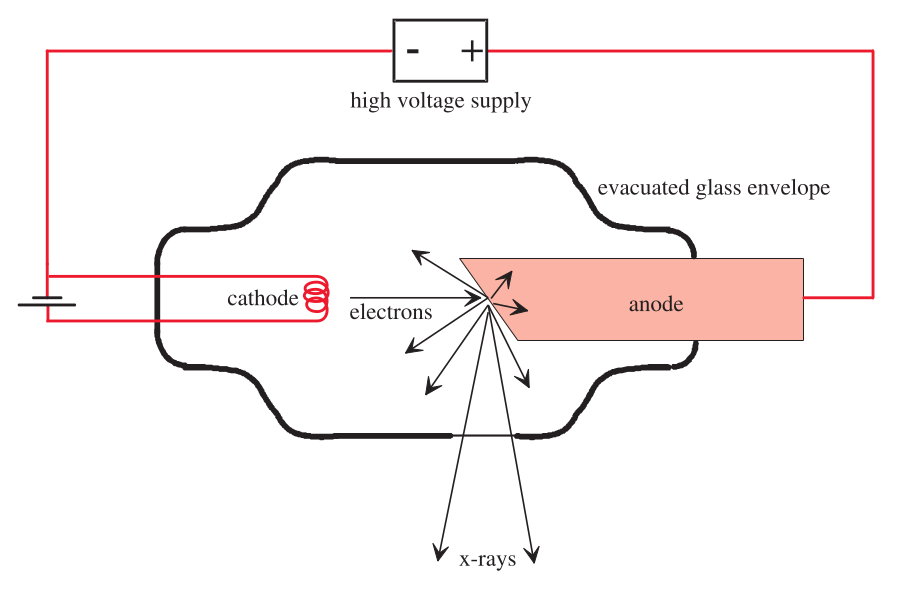
\includegraphics[width=0.8\textwidth]{figures/x_ray_tube.png}
\caption{An X-ray tube produces X-ray photons by firing projectile electrons from a cathode to an anode. \emph{Source: G.~Michael (2001) \cite{michael2001x}}}
\label{fig:x_ray_tube}
\end{figure}

Bremsstrahlung radiation is the result of projectile electrons deaccelerating due to the electrostatic field produced by nucleus of the target. The kinetic energy of the projectile electrons is then converted to electromagnetic radiation to produce X-ray radiation. As a result, the photon energies in bremsstrahlung radiation is  a continuous spectrum and can range up to the maximum kinetic energy of the projectile electrons \cite{michael2001x}.

Characteristic radiation is due to projectile electrons colliding with electrons in the target atom and ionizing them. This produce vacancies in the electron shell and emits X-ray photons when the electrons in the target atom drops down back to the ground state. The energy of the emitted radiation is monoenergetic and depends on the binding energy of the target's atoms \cite{michael2001x}.

A typical energy spectrum of X-ray photons emitted from an X-ray tube is as shown in Figure \ref{fig:x_ray_spectrum}. The energy spectrum consist of both bremsstrahlung and characteristic radiation \cite{michael2001x}.

\begin{figure}
\centering
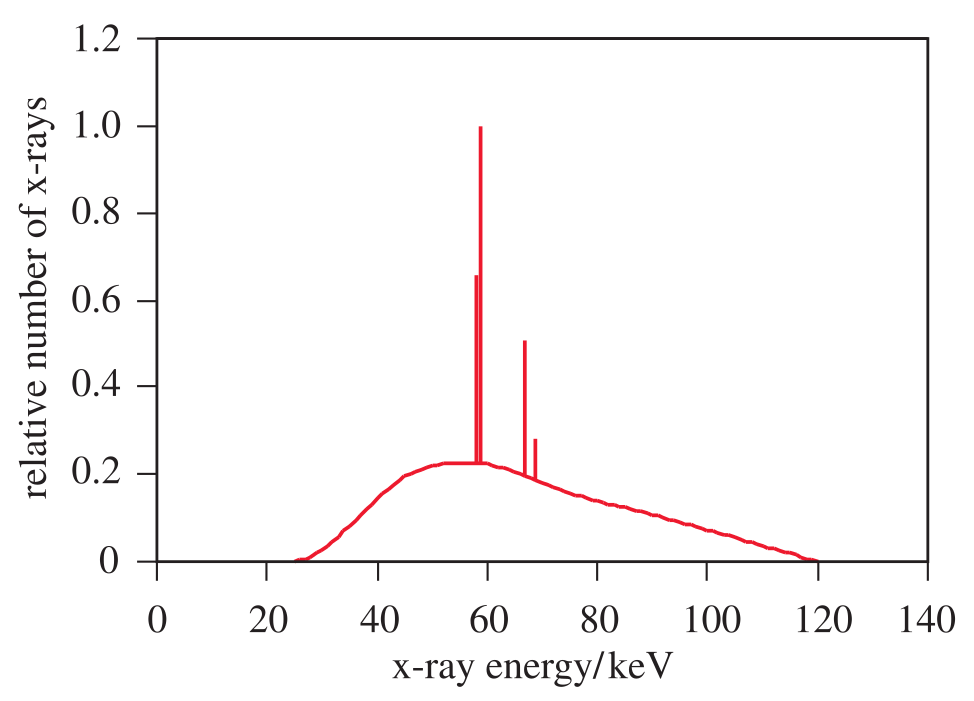
\includegraphics[width=0.8\textwidth]{figures/x_ray_spectrum.png}
\caption{A typical energy spectrum of X-ray photons emitted from an X-ray tube. The continuous spectrum is the result of Bremmsstrahlung radiation. The peaks are the result of characteristic radiation. \emph{Source: G.~Michael (2001) \cite{michael2001x}}}
\label{fig:x_ray_spectrum}
\end{figure}

The voltage, the energy per charge, and current, the rate of charge, can be varied in the X-ray tube to produce different energy spectrums and rate of X-ray emittion. This can vary the results produced when collecting CT data \cite{cantatore2011introduction}. Another important factor is the focal spot size because smaller spot sizes produce sharper edges. Larger spot sizes produce unsharp results and this is know as the penumbra effect, as shown in Figure \ref{fig:x_ray_penumbra}. However spot sizes too small can produce concentrated heat \cite{welkenhuyzen2009industrial}.

\begin{figure}
\centering
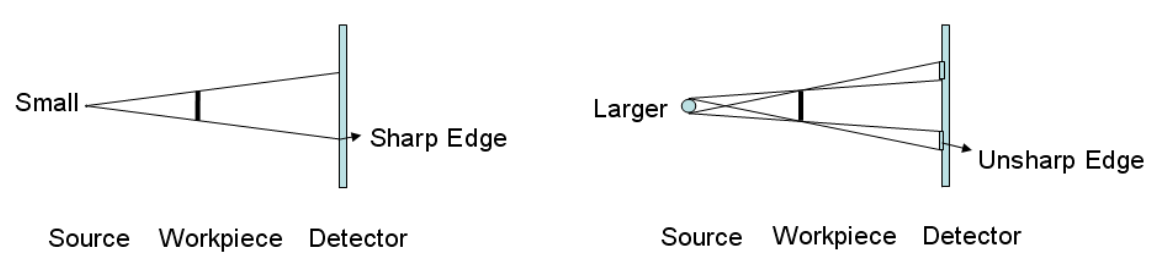
\includegraphics[width=1\textwidth]{figures/x_ray_penumbra.png}
\caption{Larger focal spot sizes produces unsharp results. This is know as the penumbra effect. \emph{Source: F.~Welkenhuyzen et al.~(2009)\cite{welkenhuyzen2009industrial}}}
\label{fig:x_ray_penumbra}
\end{figure}

\section{X-Ray Interactions}
X-ray radiation emitted by the X-ray tube are projected onto the sample and interacts with it in a number of ways \cite{cantatore2011introduction}.

The sample can effectively absorb X-ray radiation via the photoelectric effect or pair production \cite{cantatore2011introduction}. In the photoelectric effect, the X-ray photons transfers all its energy to a bounded electron and ejects it from the atom \cite{millikan1916direct}. In pair production, the X-ray photons converts into an electron-position pair by interacting with the Coulomb field of the sample's atomic nucleus \cite{hubbell2006electron}.

X-ray photons can be scattered by the sample. This happens when X-ray photons collide inelastically with and transfers it's energy to the sample's electrons. This process is know as Compton scattering \cite{compton1923quantum}.

The attenuation (decrease in X-ray intensity from $I_0$ to $I_1$) when propagating though a material with attenuation coefficient $\mu$ and distance $x$ is given as
\begin{equation}
I_1 = I_0\euler^{-\mu x}
\end{equation}
where it was assumed the X-ray photons are monoenergetic \cite{michael2001x}. This can be extended to a continuous spectrum of X-ray energies by making $\mu$ dependent on the energy of the X-ray photons \cite{cantatore2011introduction}. In general low energy photons are more likely to be absorbed than high energy photons, this increases the average energy of the attenuated photons and can be a source of error in CT scanning. This is referred to beam hardening \cite{michael2001x}. This can be reduced by placing a thin sheet of filter to absorb low energy photons \cite{welkenhuyzen2009industrial} or by correcting it in the data analysis stage \cite{michael2001x}.

\section{Detector}
Most X-ray detectors are scintillator-photodiode detectors. The X-ray photons interact with the scintiallator material and produces visible light. The visible light is then detected by photodiodes and coverts it into electricical current \cite{michael2001x}. The detectors used in CT scanning are flat bed scanner which consist of an array of panels of photodiodes \cite{cantatore2011introduction}.

\section{Reconstruction}
The scale of the 2D images are calibrated with the use of reference standards \cite{bartscher2007enhancement}. The method used to reconstruct the 3D geometry of the sample is called the filtered back-projection \cite{michael2001x}. The mathematics can be reviewed in \cite{brooks1976principles}.

\chapter{Exploratory Data Analysis}
\section{Summary Statistics}
A dataset was given for this project. It consists of 100 realizations of an X-ray image of a cuboid with its vertices in the middle, taken using an X-ray detector. These images were 1\,996$\times$1\,996 pixels in size and have a colour depth of 16 bits. A sample of them can be viewed in Figure \ref{fig:block_montage}.

\begin{figure}
\centering
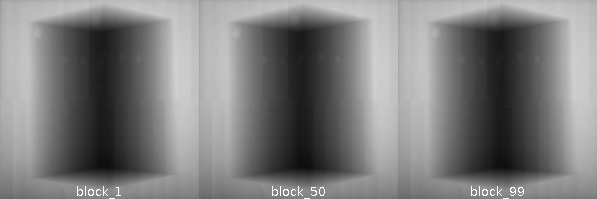
\includegraphics[width=1\textwidth]{figures/block_montage.jpg}
\caption{The 1st, 50th and 99th image in the dataset of an X-ray image of a cuboid.} 
\label{fig:block_montage}
\end{figure}

\subsection{Histogram}
The distribution of the grey values of all the pixels in the data set is shown in Figure \ref{fig:block_histogram}. It was observed that there were 3 distinct peaks in the histogram at $\sim2\times10^4$, $\sim4\times10^4$ and $\sim5\times10^4$. By doing a threshold, as shown in Figure \ref{fig:block_histogram}, it was clear that the main 3 sources of the grey values were the sample, the background and the foam holder at the bottom of the image.

\begin{figure}
\centering
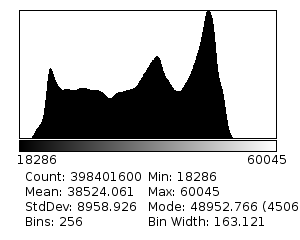
\includegraphics[width=0.5\textwidth]{figures/block_histogram.png}
\caption{Histogram of the grey values of all the pixels in the 100 images in the dataset. The grey values range from 18\,286 to 60\,045.}
\label{fig:block_histogram}
\end{figure}

\begin{figure}
	\centering
	\begin{subfigure}[b]{0.45\textwidth}
		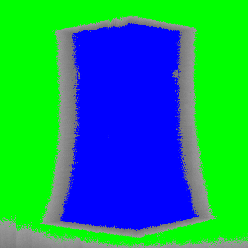
\includegraphics[width=\textwidth]{figures/block_threshold.png}
		\caption{Threshold pixels}
	\end{subfigure}
	\begin{subfigure}[b]{0.45\textwidth}
		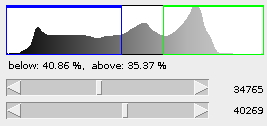
\includegraphics[]{figures/block_threshold_histogram.png}
		\caption{Histogram}	
	\end{subfigure}
	\caption{A threshold was selected to highlight pixels with different grey values. Blue: grey values less than 34\,765. Green: grey values more than 40\,269.}
	\label{fig:block_threshold}
\end{figure}

\subsection{Time Series}
The mean and standard error of the grey values for each of the 100 images were taken and plotted as a time series as shown in Figure \ref{fig:timeSeries}. There was evidence of dependence between samples by looking the sample autocorrelation plots as shown in Figure \ref{fig:timeSeries_acf_pacf}. Because there was a peak at lag 1 in the sample partial autocorrelation plot, the time series could be modelled using an autoregressive model with one parameter.

\begin{figure}
	\centering
	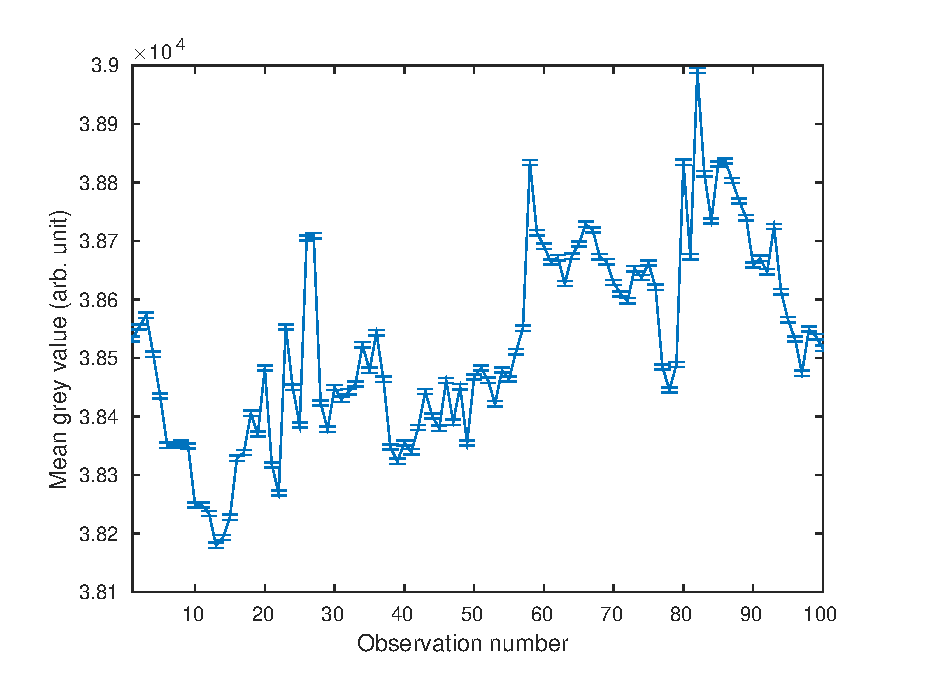
\includegraphics[width=0.75\textwidth]{figures/initial_timeSeries.eps}
	\caption{The mean and standard error of all the pixel grey values for each image.}
	\label{fig:timeSeries}
\end{figure}

\begin{figure}
	\centering
	\begin{subfigure}[b]{0.45\textwidth}
		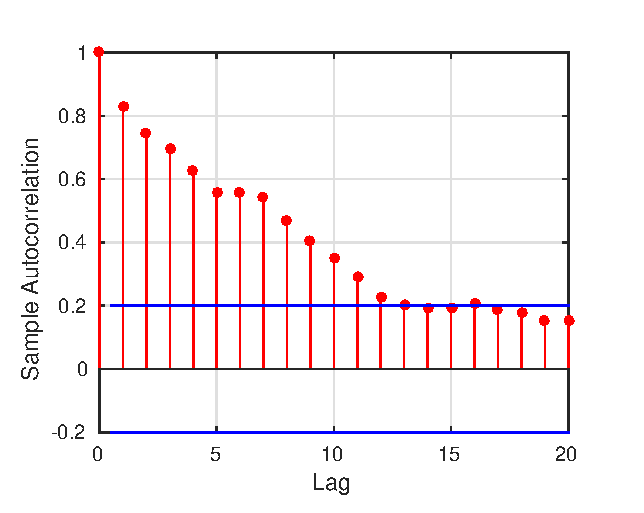
\includegraphics[width=1\textwidth]{figures/initial_acf.eps}
		\caption{Sample autocorrelation}
	\end{subfigure}
	\begin{subfigure}[b]{0.45\textwidth}
		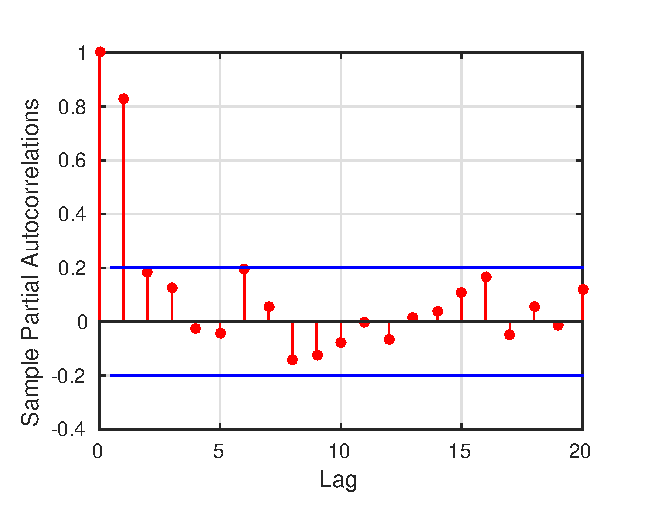
\includegraphics[width=1\textwidth]{figures/initial_pacf.eps}
		\caption{Sample partial autocorrelation}
	\end{subfigure}
	\caption{Sample autocorrelation and partial autocorrelation of the mean grey values time series.}
	\label{fig:timeSeries_acf_pacf}
\end{figure}

\subsection{Distribution of Individual Pixels}
The mean and standard deviation for each pixel's grey value was estimated and as shown in Figure \ref{fig:initial_mean_std}. Both supervised and unsupervised learning can be used to model the mean and variance relationship of the grey values.

\begin{figure}
	\centering
	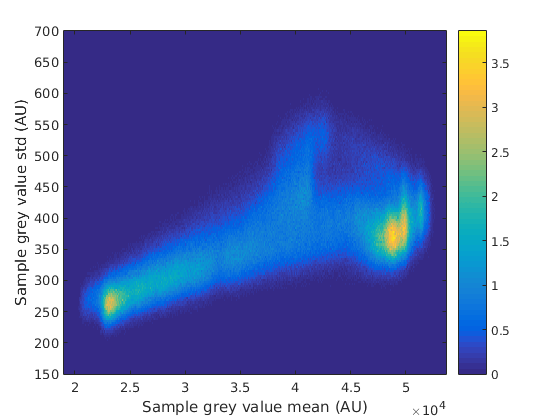
\includegraphics[width=0.9\textwidth]{figures/initial_mean_std.eps}
	\caption{Frequency density of the $1\,996^2$ pixel's grey values mean and standard deviation.}
	\label{fig:initial_mean_std}
\end{figure}

A Normal distribution was fitted on each pixel's grey values and the $\chi^2$ goodness of fit test was conducted, as shown in Figure \ref{fig:initial_fit_normal_test}. When considering the Bonferoni correction \cite{weisstein2004bonferroni} for multiple hypothesis testing, the Normal distribution appeared to be a good fit because only 9 pixels have $p$ values less than 10\%. In addition, these significant pixels did not seem to cluster and appear random in space. When ignoring the Bonferoni correction, there was a suspicious patch of low $p$ values on the bottom right.

\begin{figure}
\centering
	\begin{subfigure}[b]{0.75\textwidth}
		\includegraphics[width=1\textwidth]{figures/initial_p.eps}
		\caption{$p$ values}
	\end{subfigure}
	\begin{subfigure}[b]{0.75\textwidth}
		\includegraphics[width=1\textwidth]{figures/initial_p_log10.eps}
		\caption{$\log_{10} p$ values}
	\end{subfigure}
	\caption{$p$ values from the $\chi^2$ goodness of fit test on fitting the Normal distribution on the grey values for each pixel. In b) circled are pixels with $p$ values less than 10\%, corrected for multiple hypothesis testing using the Bonferroni correction.}
	\label{fig:initial_fit_normal_test}
\end{figure}

\section{Principal Component Analysis}
By estimating the covariance matrix of the individual pixel's grey values, sources of (orthgonal) variance can be estimated. This can be done investigating eigendecomposition representation of the sample covariance matrix. A lot of the linear algebra can be reviewed in undergraudate maths text book such as \cite{riley2006mathematical}.

\subsection{Theory}
Suppose the $p\times p$ covariance matrix $\matr{\Sigma}$ has eigenvalues $\lambda_i$ and eigenvector $\vectGreek{\phi}_i$ for $i=1,2,\dotdotdot,p$. Then the eigenvectors and eigenvalues are related by
\begin{equation}
\matr{\Sigma}\vectGreek{\phi}_i = \lambda_i\vectGreek{\phi}_i \ .
\label{eq:eigenvector_eigenvalue_forCovariance}
\end{equation}
A closure can be form by pre-multiplying both sides by $\vectGreek{\phi}_j\T$ so that
\begin{align*}
\vectGreek{\phi}_j\T \matr{\Sigma}\vectGreek{\phi}_i &= \lambda_i\vectGreek{\phi}_j\T\vectGreek{\phi}_i \\
\left(\matr{\Sigma}\T \vectGreek{\phi}_j \right)\T\vectGreek{\phi}_i &= \lambda_i\vectGreek{\phi}_j\T\vectGreek{\phi}_i \ .
\end{align*}
But given the covariance matrix is symmetric, $\matr{\Sigma}=\matr{\Sigma}\T$, and $\lambda_j$ is the corresponding eigenvalue of the eigenvector $\vectGreek{\phi}_j$, then
\begin{align*}
\left(\lambda_j\vectGreek{\phi}_j \right)\T\vectGreek{\phi}_i &= \lambda_i\vectGreek{\phi}_j\T\vectGreek{\phi}_i \\
\lambda_j\vectGreek{\phi}_j\T\vectGreek{\phi}_i &= \lambda_i\vectGreek{\phi}_j\T\vectGreek{\phi}_i \ .
\end{align*}
As long as $\lambda_i\neq\lambda_j$ for $i\neq j$, then $\vectGreek{\phi}_j\T\vectGreek{\phi}_i=0$. Therefore all eigenvalues in the covariance matrix are orthogonal to each other.

Equation \eqref{eq:eigenvector_eigenvalue_forCovariance} can be extended to include all eigenvectors and eigenvalues such that
\begin{equation}
\matr{\Sigma}
	\begin{pmatrix}
		\uparrow & \uparrow & & \uparrow \\
		\vectGreek{\phi}_1 & \vectGreek{\phi}_2 &\cdots& \vectGreek{\phi}_p \\
		\downarrow & \downarrow & & \downarrow \\
	\end{pmatrix}
=
	\begin{pmatrix}
		\uparrow & \uparrow & & \uparrow \\
		\lambda_1\vectGreek{\phi}_1 & \lambda_2\vectGreek{\phi}_2 &\cdots& \lambda_p\vectGreek{\phi}_p \\
		\downarrow & \downarrow & & \downarrow \\
	\end{pmatrix} \ .
\end{equation}
Transposing both sides
\begin{equation*}
\begin{pmatrix}
	\leftarrow\vectGreek{\phi}_1\rightarrow \\
	\leftarrow\vectGreek{\phi}_2\rightarrow \\
	\vdots \\
	\leftarrow\vectGreek{\phi}_p\rightarrow
\end{pmatrix}
\matr{\Sigma}
=
\begin{pmatrix}
	\lambda_1 & 0 & \cdots 0 \\
	0 & \lambda_2 & \cdots 0 \\
	\vdots & \vdots & \ddots \\
	0 & 0 & \cdots \lambda_p \\
\end{pmatrix}
\begin{pmatrix}
	\leftarrow\vectGreek{\phi}_1\rightarrow \\
	\leftarrow\vectGreek{\phi}_2\rightarrow \\
	\vdots \\
	\leftarrow\vectGreek{\phi}_p\rightarrow
\end{pmatrix}
\end{equation*}
but because all eigenvectors are orthogonal
\begin{equation*}
\matr{\Sigma}
=
\begin{pmatrix}
		\uparrow & \uparrow & & \uparrow \\
		\vectGreek{\phi}_1 & \vectGreek{\phi}_2 &\cdots& \vectGreek{\phi}_p \\
		\downarrow & \downarrow & & \downarrow \\
\end{pmatrix}
\begin{pmatrix}
	\lambda_1 & 0 & \cdots 0 \\
	0 & \lambda_2 & \cdots 0 \\
	\vdots & \vdots & \ddots \\
	0 & 0 & \cdots \lambda_p \\
\end{pmatrix}
\begin{pmatrix}
	\leftarrow\vectGreek{\phi}_1\rightarrow \\
	\leftarrow\vectGreek{\phi}_2\rightarrow \\
	\vdots \\
	\leftarrow\vectGreek{\phi}_p\rightarrow
\end{pmatrix} \ .
\end{equation*}
This is just a weighted sum of the outer products of the eigenvectors, therefore the eigendecomposition is
\begin{equation}
\matr{\Sigma} = \sum_{i=1}^{p} \lambda_i \vectGreek{\phi}_i \vectGreek{\phi}_i\T \ .
\end{equation}
Because this is a weighted sum, the eigenvectors with the biggest eigenvalue will be most responsible for the covariance matrix. $\vectGreek{\phi_i}$ are called the principle components.

\subsection{Methods}
The 100 images were shrunk with averaging to a size of $100\times100$ pixels using ImageJ. The sample covariance matrix, of the pixel's grey values, was calculated using the maximum likelihood estimator so that the 6 eigenvectors with the biggest eigenvalues can be obtained. Using 1\,600 bootstrap samples, the sampling distribution of the 6 eigenvalues were sampled.

\subsection{Results}
Figure \ref{fig:initial_PC_eigenvalues} shows the first 6 of the diagonal of the outer product of the individual principle components, they represent the normalised main sources of variance. It was observed that on the first and second principle components, there are sources of variance in the bottom right and top right of the image. This could imply that the sources of variance are not uniformly distributed in the background.

The sampling distribution of the eigenvalues are shown in Figure \ref{fig:initial_PC_eigenvalues}. Quite clearly there were 2 significant sources of variance because the eigenvalues of the first 2 principle components were much larger than zero when comparing it with its interquartile range.

\begin{figure}
	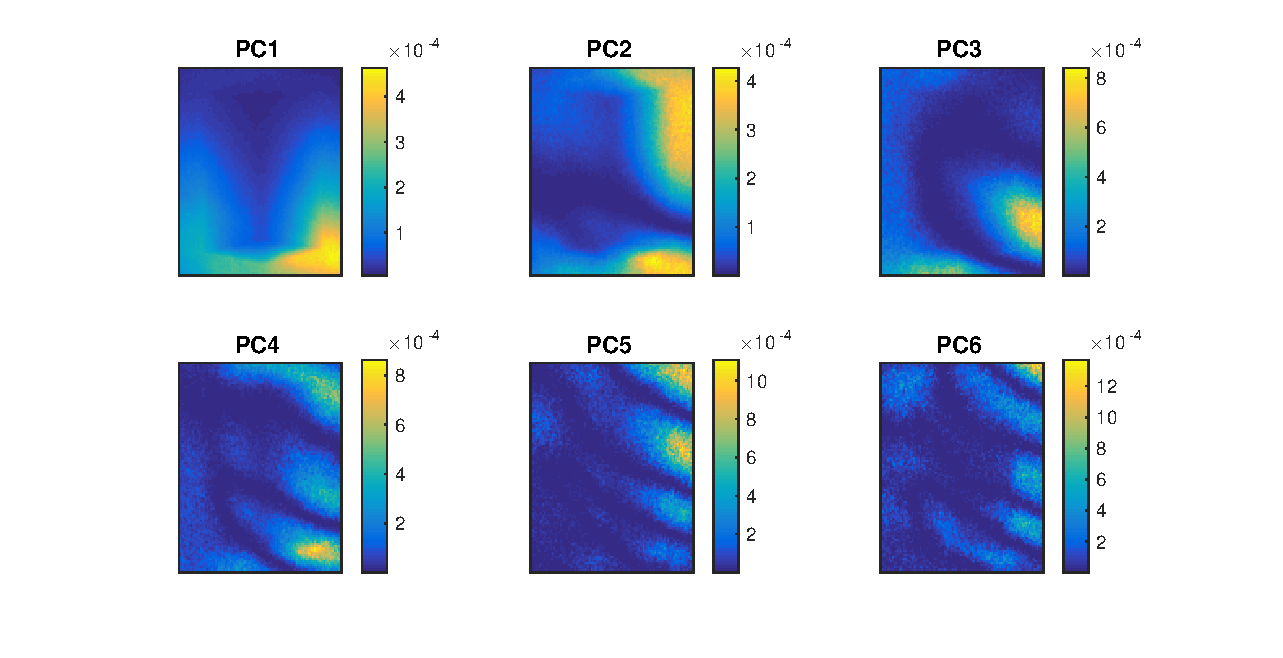
\includegraphics[width=\textwidth]{figures/initial_PCvariance.eps}
	\caption{Normalised variance due to the principle components (1 to 6). The values of all the pixels in the figures equal to 1.}
	\label{fig:initial_PCvariance}
\end{figure}
\begin{figure}
	\centering
	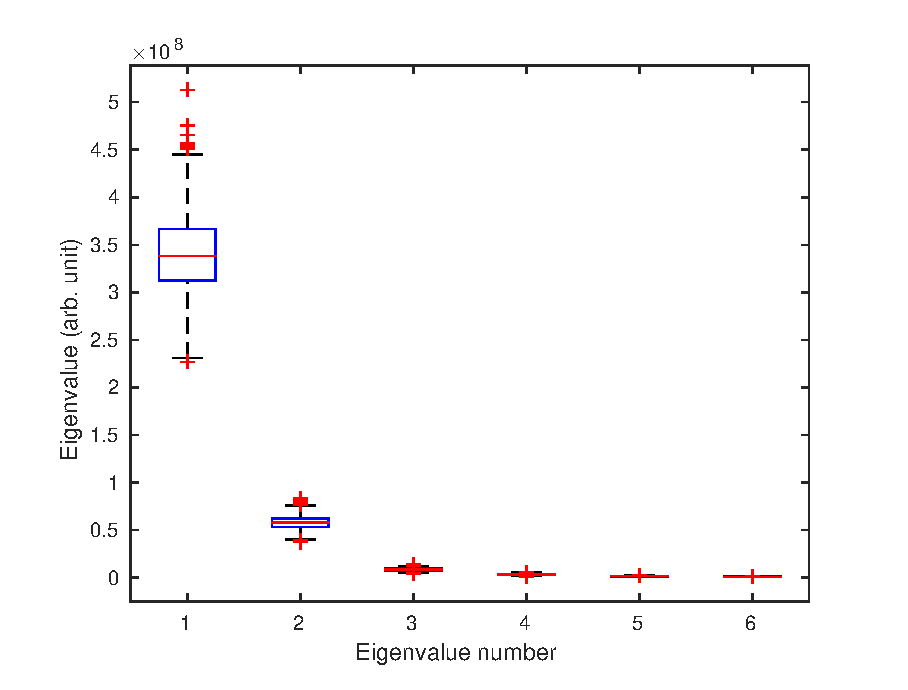
\includegraphics[width=0.7\textwidth]{figures/initial_PC_eigenvalues.eps}
	\caption{Eigenvalues of the sample covariance matrix. 1\,600 bootstrap samples were used.}
	\label{fig:initial_PC_eigenvalues}
\end{figure}

\section{Factor Analysis}
\subsection{Theory}
\subsection{Methods}
\subsection{Results}
\chapter{Mean and Variance Relationship}


\bibliographystyle{unsrt}
\bibliography{bib}
\end{document}